%Apendice B
%
\chapter{Tablas de carga de la máquina de fatiga}
\label{ch:anexo_b}

\section{Tabla de cargas original}
\label{sec:anexob1}

La siguiente tabla es la que se utiliza actualmente para realizar los ensayos de fatiga en flexión. 

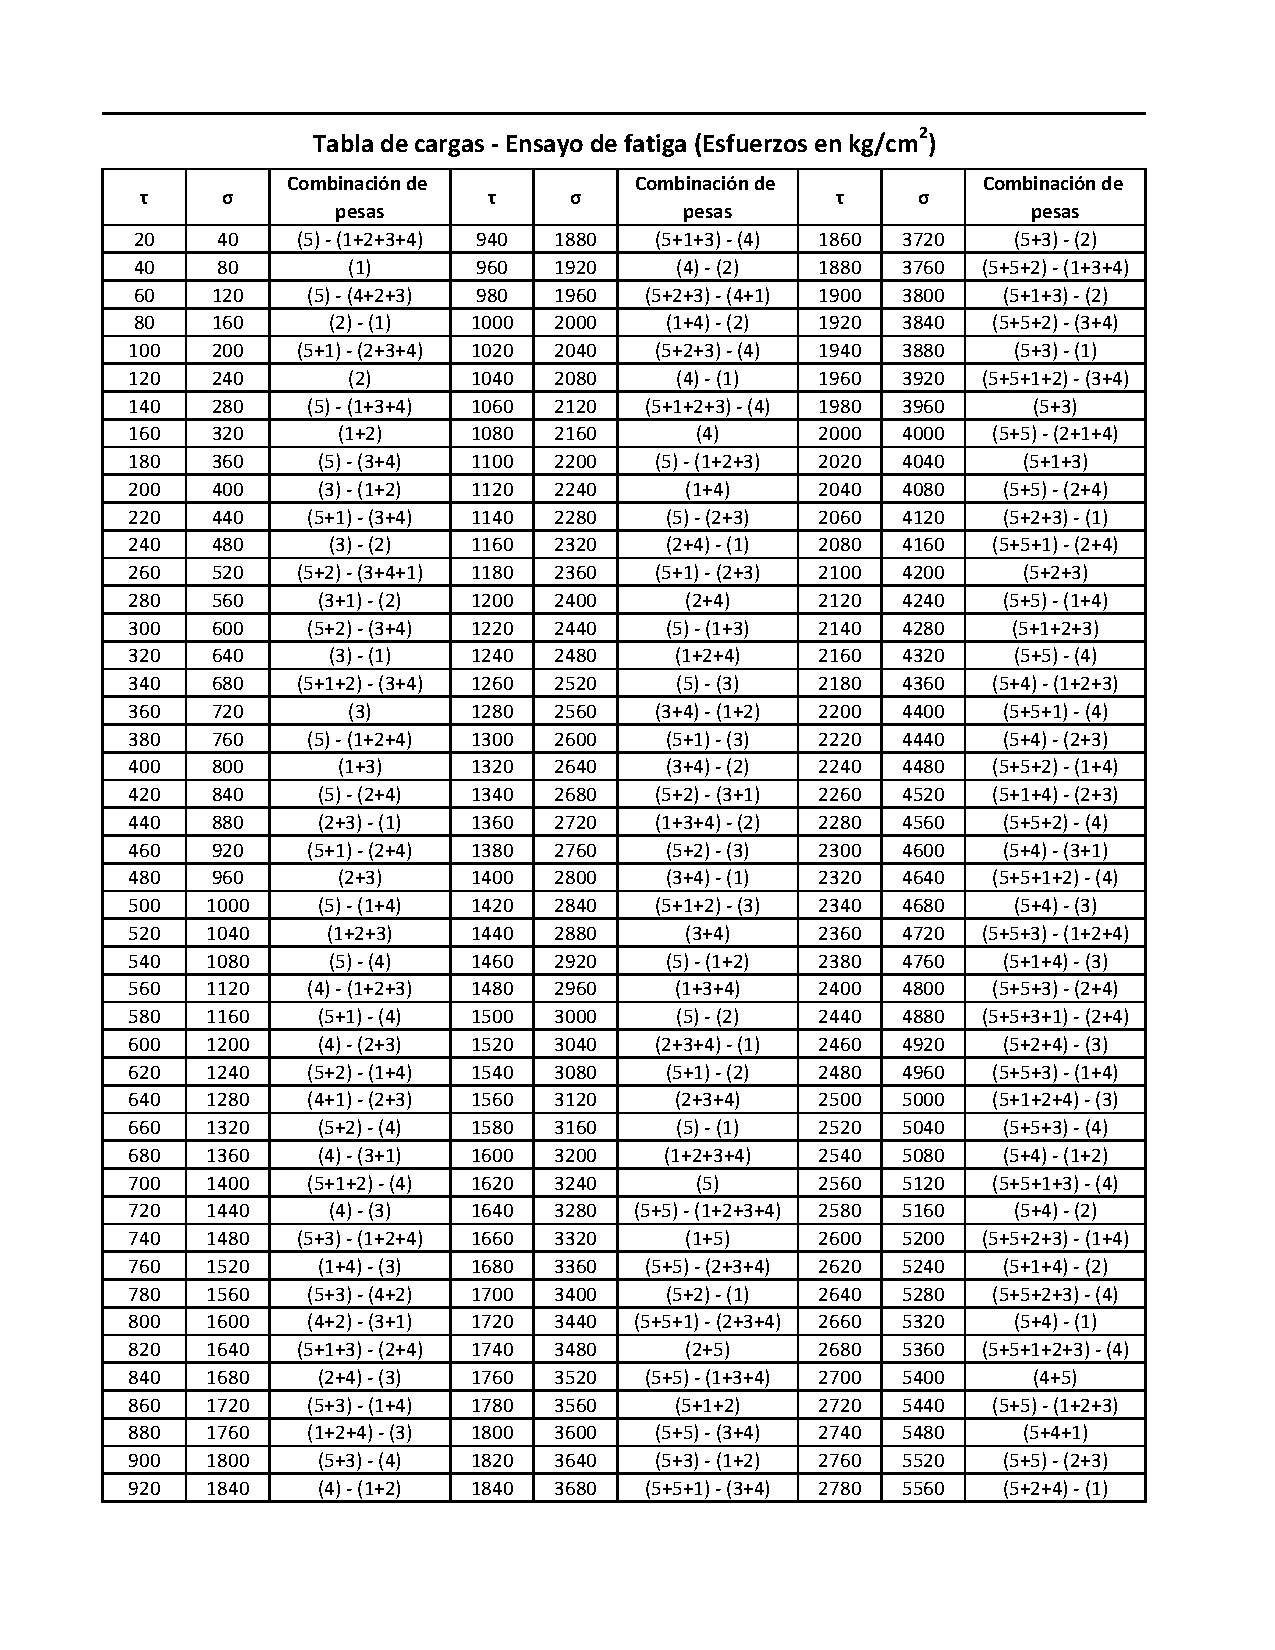
\includepdf[pages=-]{Anexos/anexo_b1.pdf}

\section{Tabla de cargas propuesta}
\label{sec:anexob2}

Esta nueva tabla es la propuesta que emana de los resultados del trabajo realizado. Los esfuerzos de cortante máximo y de von Mises se toman a partir del punto $R$, según la referencia \ref{fig:diag_pqr}. Además, se añaden las columnas $m_1$ y $m_2$ que corresponden a la masa total de cada combinación. Por último, se agrega la columna  ``\textit{Fuerza}'' que es la fuerza máxima $F_{max}$ obtenida en el modelo de vibraciones para cada combinación de contrapesos.

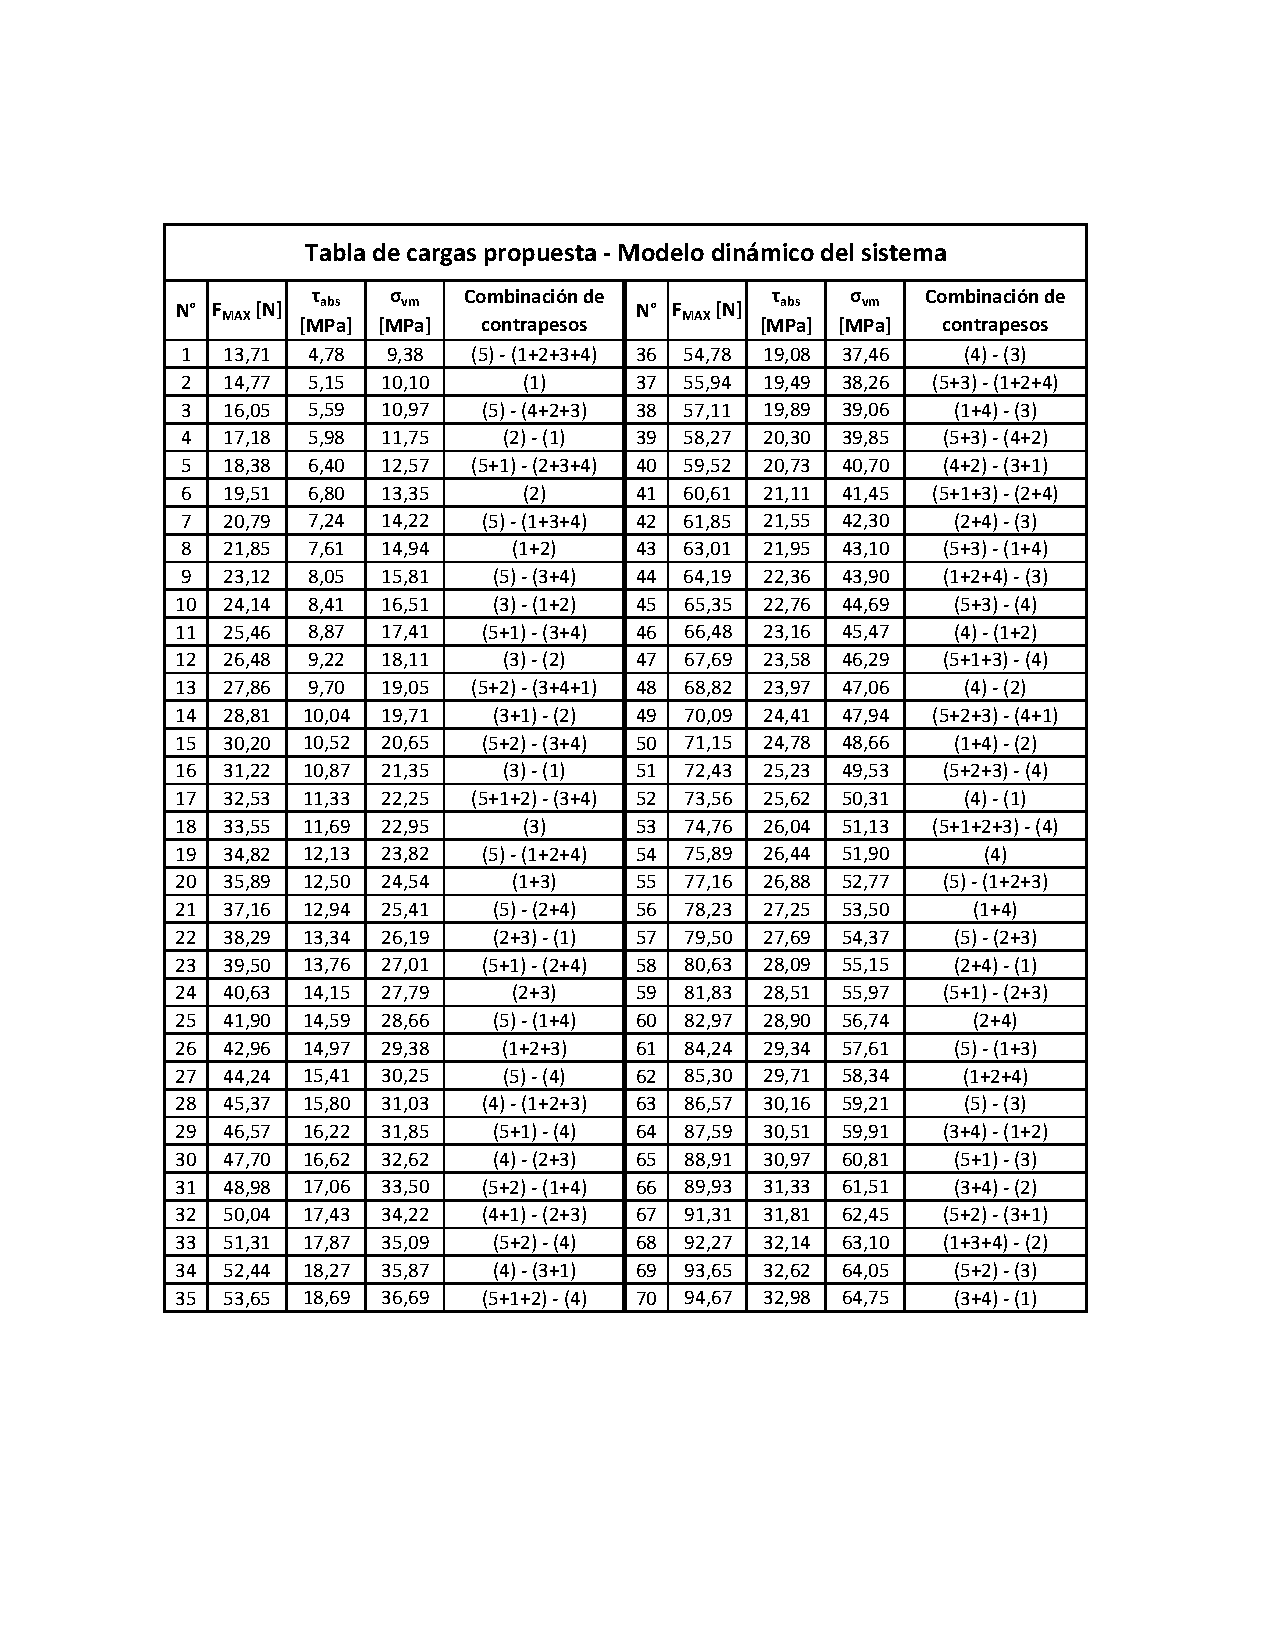
\includepdf[pages=-]{Anexos/anexo_b2.pdf}